\documentclass[12pt]{article}

\usepackage[utf8]{inputenc}
\usepackage[T1]{fontenc}
\usepackage{amsmath, amssymb}
\usepackage{graphicx}
\usepackage{booktabs}
\usepackage{caption}
\usepackage[margin=1in]{geometry}
\usepackage{natbib}
\usepackage{hyperref}
\graphicspath{{figures/}}

\title{The Effect of Timestep Size on the Accuracy of Euler's Method in Simulating Free-Fall Motion}
\author{Arnav Deopura}
\date{\today}

\begin{document}
\maketitle

\section{Introduction}

Many physical systems all over the universe are defined by differential equations. Although some differential equations have analytical solutions, many are too complex to solve, which is where numerical methods can aid. Numerical methods provide approximate solutions that may not be exact, but are much easier to solve and are usually sufficient for most real-world problems. Therefore, they are widely used in multiple fields, including but not limited to, physics, engineering, chemistry, biology, and many other scientific areas.

One of the simplest and fastest of these numerical methods is the Euler method, named after the Swiss mathematician Leonhard Euler. Euler's method is a first-order numerical method that uses information about the local derivative to take small steps forward, simulating a path. Although computationally fast and simple, its accuracy depends greatly on the chosen timestep \citep{gilat2013}. Timestep must be chosen wisely to prevent both truncation errors and round-off errors, as well as save time.

Previous studies have compared and applied numerical methods to a variety of disciplines. For instance, \citet{kaniz2025} found that higher-order numerical methods such as Runge-Kutta 4 (RK4) generally produce less error than lower-order methods such as Euler when presenting a two-compartment pharmacokinetic model, which is a differential equation. In addition, \citet{mungandenker2012} discuss how it was necessary for them to use numerical integration to simulate a ball shooting out of a musket under general conditions due to differential equations failing to accommodate if the initial position and velocity is not zero. These studies highlight the importance of understanding numerical methods, their accuracies, and their applications.

In this project, we aim to investigate how timestep size affects the accuracy of Euler's method when simulating free-fall motion under constant gravitational acceleration. Numerical solutions generated under this method will be compared and analyzed against the analytical solution, and the errors will be further analyzed for several timestep values. We predict that smaller timesteps will produce more accurate approximations and result in overall less numerical errors when compared with the analytical solution.

\section{Methods}

To investigate the accuracy of Euler's method, a simulation made using Python was developed.
This simulation models a theoretical ball being dropped. The initial height of this object is placed at 100.0 meters with its initial velocity at 0.0 meters per second to represent the ball being dropped from rest. The only force acting on this object is a simulated gravitational force that pulls the ball down by accelerating at $-9.81 \text{ m/s}^2$. Other forces such as air resistance were neglected due to the focus on isolating the numerical error of Euler's method.

To establish a baseline for exact accuracy, the true position of the falling object at any given time was calculated using the standard kinematic equation for uniform acceleration:
\begin{equation}
y(t) = y_0 + v_0 t + \frac{1}{2} g t^2
\label{eq:kinematic}
\end{equation}
Where $y_0$ is the initial height, $v_0$ is the initial velocity, $g$ is the gravitational acceleration, and $t$ is the elapsed time since the object is dropped.

The numerical approximation was executed using the forward Euler method, as mentioned before. In this method, instead of calculating the continuous path, the simulation advances in discrete time increments, or timestep ($\Delta t$). For each step, the algorithm updates the object's velocity and position sequentially using the following linear approximations:
\begin{align}
y_{n+1} &= y_n + v_n \,\Delta t \label{eq:euler-y}\\
v_{n+1} &= v_n + g \,\Delta t \label{eq:euler-v}
\end{align}
The simulation ran continuously through a loop, updating the values (time, position, and velocity) until the object's height reaches zero, which in the real world would mean that the ball has hit the ground.

To test the hypothesis regarding timestep size, the simulation was automated to run across five different timestep values: 0.01s, 0.05s, 0.1s, 0.5s, and 1.0s. During each execution, the code calculated both the numerical solution as well as the exact analytical position at every individual timestep. The absolute position error was recorded at each increment. Once a simulation finished, the algorithm utilized the \textit{NumPy} library to calculate the statistical mean error and identify the maximum absolute error for that specific timestep size. Finally, the data was then visualized using the \textit{Matplotlib} library to plot the comparative trajectories, the accumulation of error over time, and the relationship between timestep size and total simulation error.

\section{Results}

The simulation successfully modeled the free-fall motion across all five designated timesteps, revealing a direct correlation between the size of the timestep and the magnitude of the position error. The numerical data showed that the smallest timestep ($\Delta t = 0.01$s) produced the most accurate approximation, having a mean position error of 0.1113 meters and a maximum error of 0.2222 meters when reaching $y=0$ (ground level). As the timestep increased, however, the error grew significantly. At $\Delta t = 0.1$s, the mean error increased around tenfold compared to $\Delta t = 0.01$s, being 1.1527 meters, with a maximum error of 2.2563 meters. At the largest timestep tested, $\Delta t = 1.0$s, the mean error resulted to be 17.1675 meters with a maximum error of 29.4300 meters. These results, along with the values for the remaining timesteps, are summarized in Table~\ref{tab:results}.

\begin{table}[h]
\centering
\caption{Mean and maximum position error as a function of timestep size.}
\label{tab:results}
\begin{tabular}{ccc}
\toprule
Timestep (s) & Mean Error (m) & Max Error (m) \\
\midrule
0.01 & 0.1113  & 0.2222  \\
0.05 & 0.5641  & 1.1159  \\
0.10 & 1.1527  & 2.2563  \\
0.50 & 6.7444  & 12.2625 \\
1.00 & 17.1675 & 29.4300 \\
\bottomrule
\end{tabular}
\end{table}

Graphical analysis of the trajectories (Figure~\ref{fig:fig1}) illustrated that the Euler method constantly overestimates the height of the falling object compared to the analytical trajectory. Additionally, tracking the error of a single drop (Figure~\ref{fig:fig2}) demonstrated that position error accumulates continuously and linearly as time progresses. Finally, plotting the aggregate data (Figure~\ref{fig:fig3}) confirmed a linear relationship between the timestep size and both the mean and maximum error values.

\begin{figure}[h]
\centering
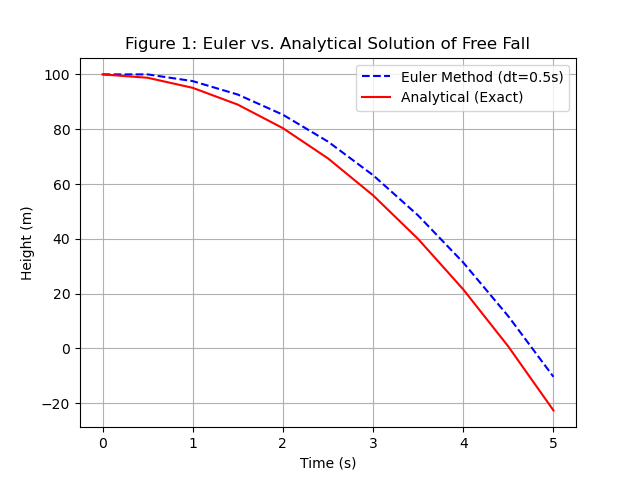
\includegraphics[width=0.8\textwidth]{Figure_1_dt_0_5.png}
\caption{Euler method approximation vs. the analytical solution for free-fall height over time ($\Delta t = 0.5$s).}
\label{fig:fig1}
\end{figure}

\begin{figure}[h]
\centering
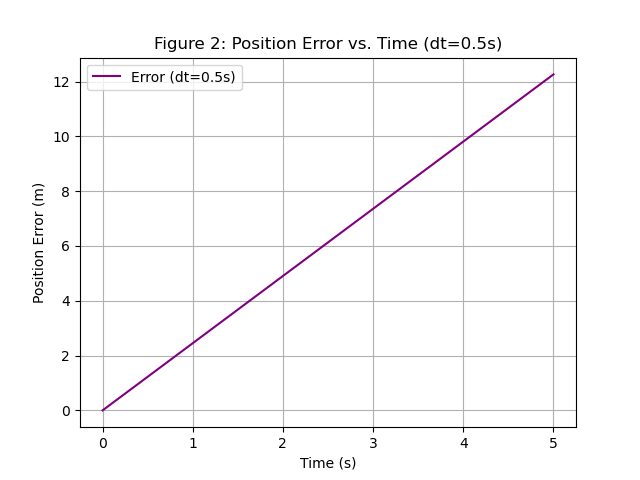
\includegraphics[width=0.8\textwidth]{Figure_2_dt_0_5.png}
\caption{Position error accumulation over time for a single simulation run ($\Delta t = 0.5$s).}
\label{fig:fig2}
\end{figure}

\begin{figure}[h]
\centering
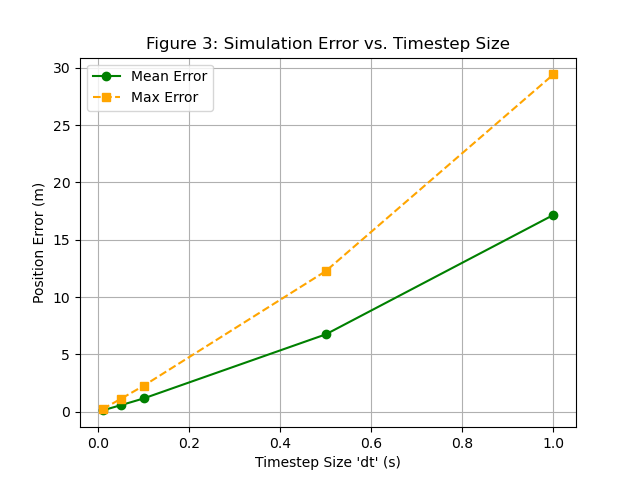
\includegraphics[width=0.8\textwidth]{Figure_3.png}
\caption{Mean and maximum position error as a function of timestep size.}
\label{fig:fig3}
\end{figure}

\section{Discussion}

The results of this simulation strongly support the initial hypothesis: as the timestep grows larger, Euler's method becomes increasingly less accurate when compared to the analytical solution. The consistent overestimation of the ball's height when using Euler can be explained by the fundamental mechanics of the method, as Euler calculates the new position by assuming that the object's velocity remains constant for the full duration of a single timestep. However, in reality, gravitational acceleration acts continuously, speeding up the ball at every fraction of a second. Since the numerical simulation calculates the distance fallen using the previous velocity at the start of the step, the simulated object does not travel as far downward as it should. This lag creates a truncation error that compounds upon itself at every step, causing the linear accumulation shown in Figure~\ref{fig:fig2}.

Furthermore, the data explicitly proves that Euler's method is a first-order numerical method, meaning the global error is proportional to step size. For instance, when the timestep was increased by a factor of ten from 0.01s to 0.1s, the mean and maximum errors correspondingly increased by a factor of approximately ten. While using smaller timesteps drastically increases accuracy, it forces the computer to do more calculations, which may become troublesome when working with complex simulations and programs. This highlights how researchers must carefully balance the trade-off between mathematical accuracy and computational efficiency. As seen in the pharmacokinetic models and musket simulations from previous literature, understanding the limitations of first-order methods such as Euler is critical to ensure that a simulation remains physically realistic.

\section{Conclusion}

In essence, this project successfully quantified the effect of timestep size when using Euler's method while simulating continuously accelerating physical systems. By comparing numerical approximations of free-fall motion against exact analytical solutions, it was determined that position error scales linear with the chosen timestep, confirming that Euler is indeed a first-order numerical method. Since the algorithm relies on discrete steps of constant velocity, it inherently underestimates downward displacement, leading to accumulating position errors that severely impact the simulation at larger timesteps. Ultimately, while Euler's method provides a fast and highly accessible foundation for solving complex differential equations, it requires the careful selection of an adequate small timestep to mitigate truncation errors from compromising the results.

\bibliographystyle{apalike}
\bibliography{references}

\end{document}
